% geni_4.tex - GENI Lab 4 for Cloud Computing class (Spring 2015)
% Chanmann Lim - April 2015

\documentclass[a4paper]{article}

\usepackage[margin=1 in]{geometry}
\usepackage{listings}
\usepackage{graphicx}
\usepackage{float}

\begin{document}
\title{CS 7001-03: Report for Lab 4: InterCloud Web Services for OpenStack\-based Cloud Orchestration}
\author{Chanmann Lim\\ 
	\texttt{cl9p8@mail.mail.missouri.edu}}
\date{April 21, 2015}
\maketitle

% ---------------------------------------- 1 ----------------------------------------
\paragraph{1. } Screenshot of the "Network Topology" in CloudLab: \\
\begin{figure}[H]
  \centering
    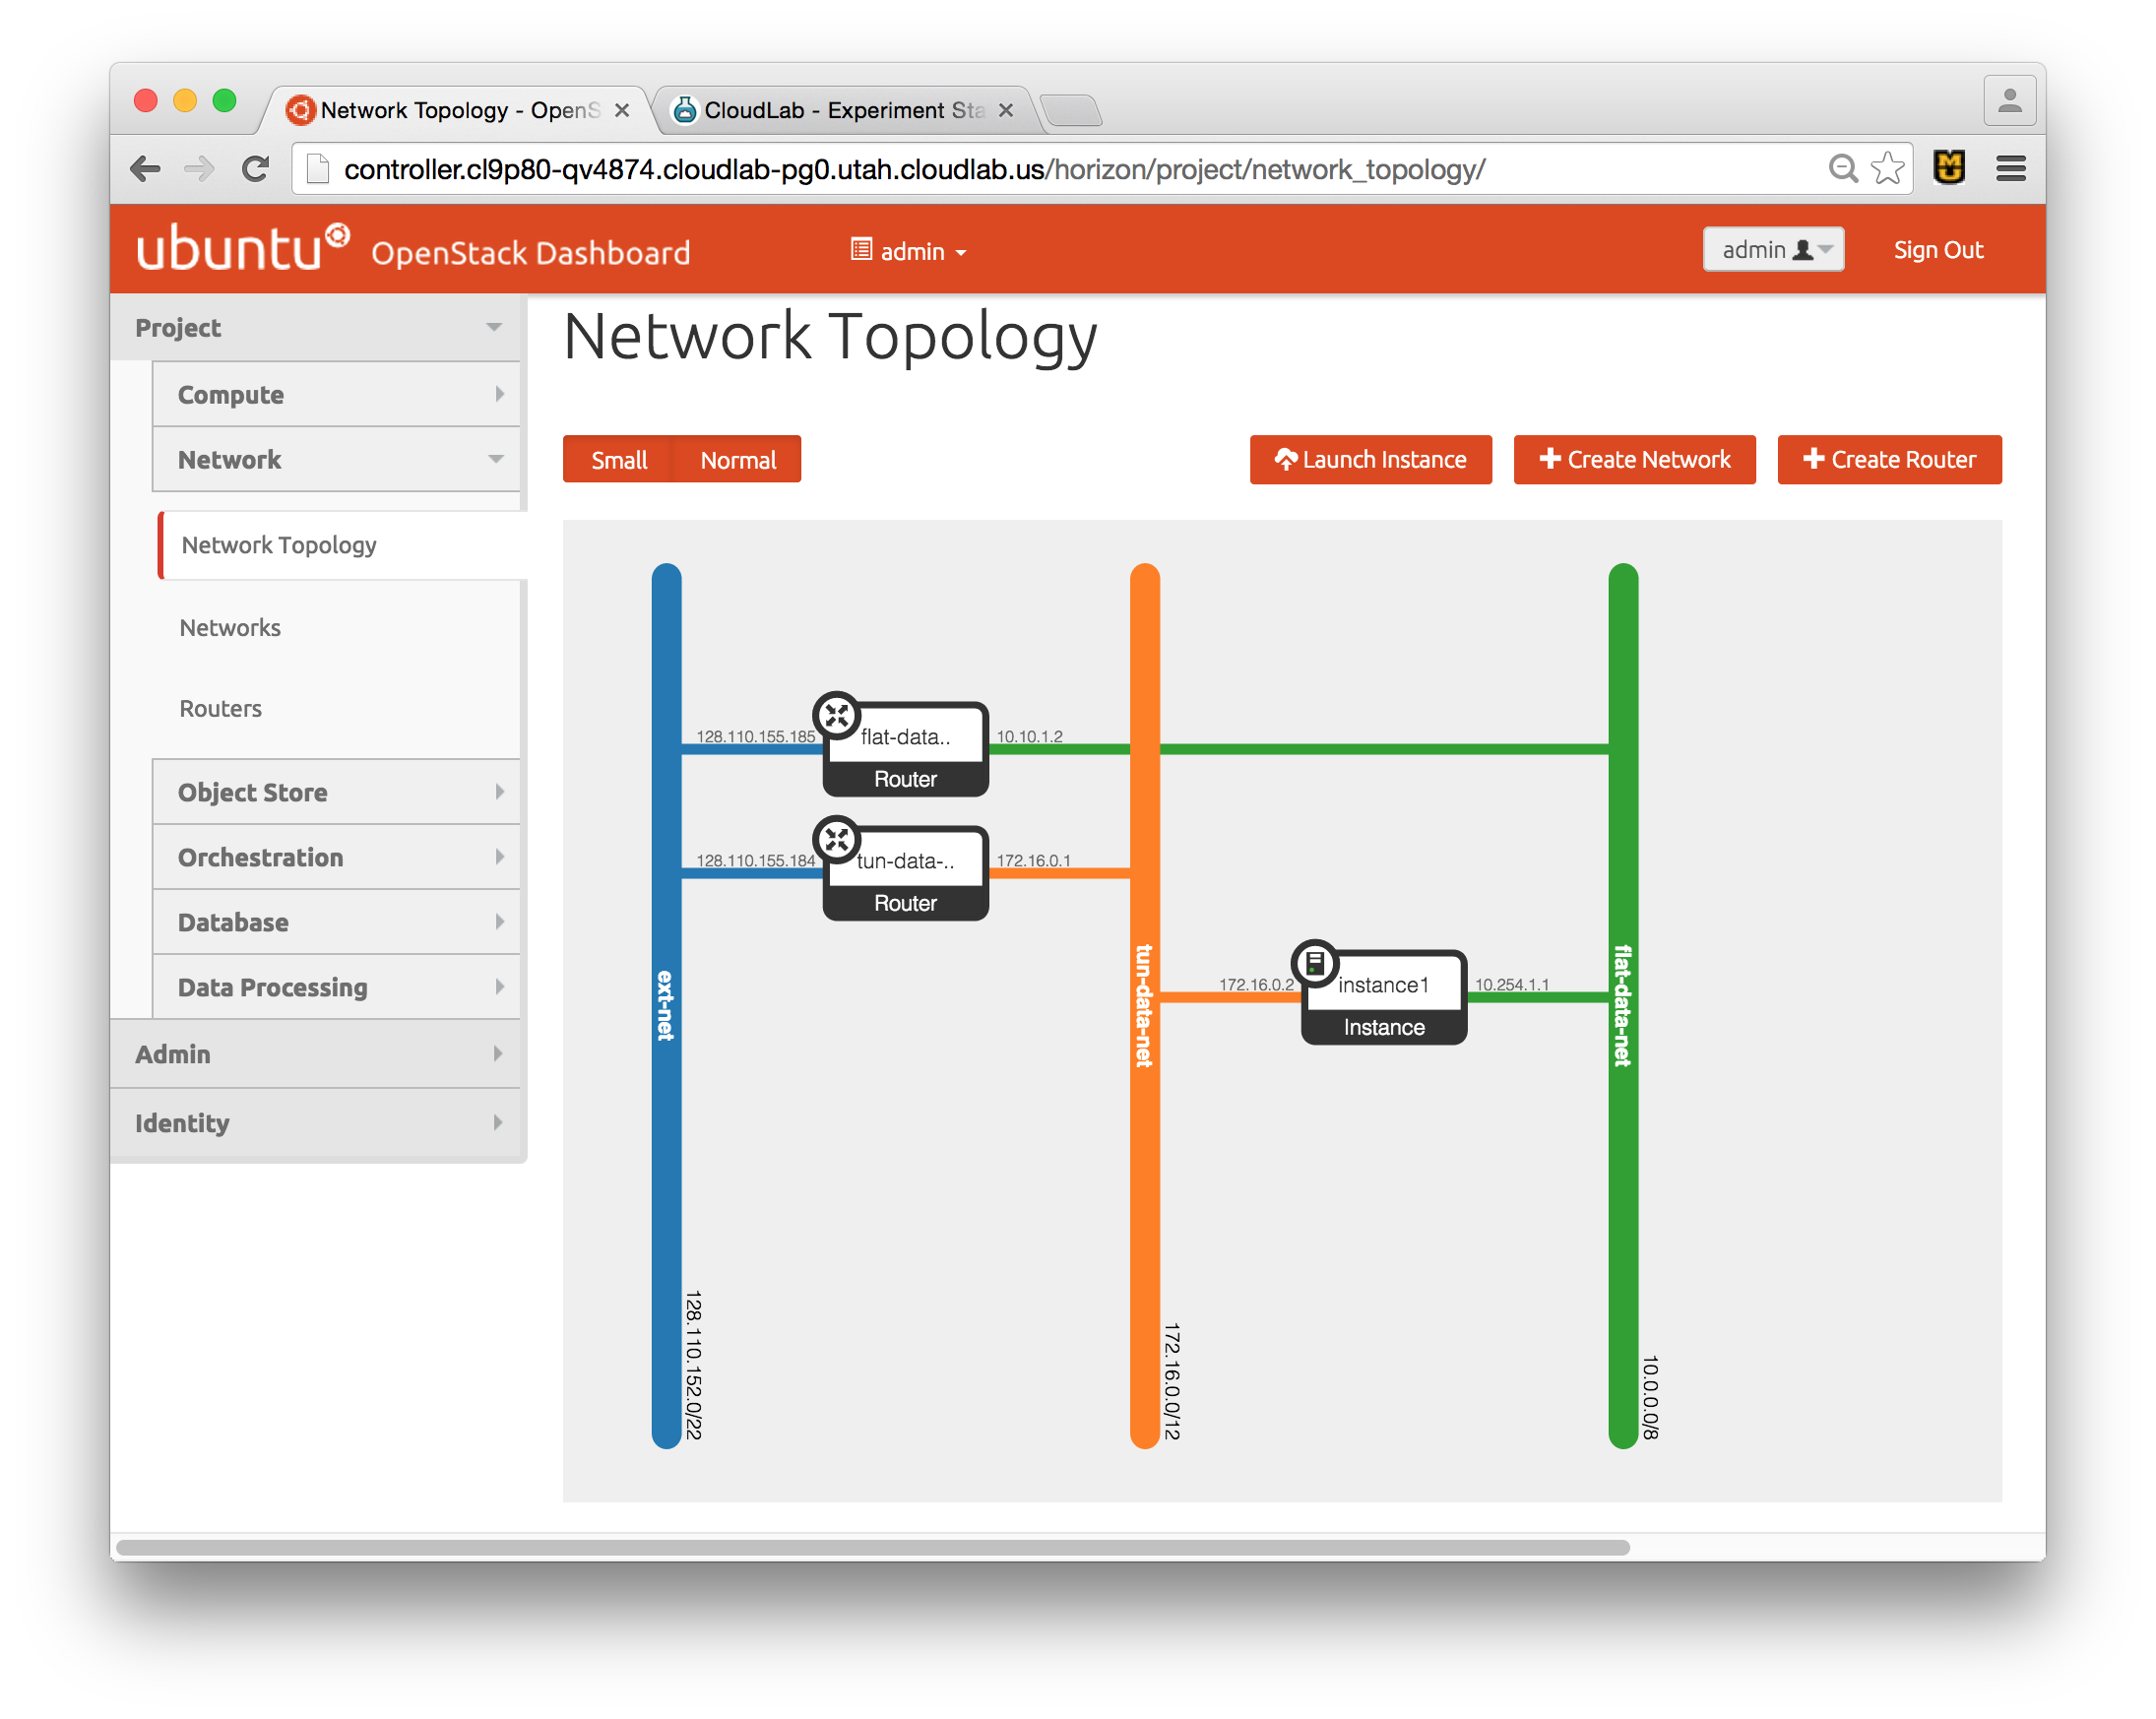
\includegraphics[scale=.37]{net_topo.png}
  \caption{Network Topology in CloudLab}
\end{figure}

The "Network Topology" tab under the Network section in the above Figure shows the three networks represented by three columns in different colors connected with each others through two routers and a newly launched instance connected to two networks namely "flat-data-net" and "tun-data-net". 

% ---------------------------------------- 2 ----------------------------------------
\paragraph{2. } Screenshot of the "controller" node's MAC address: \\
\begin{figure}[H]
  \centering
    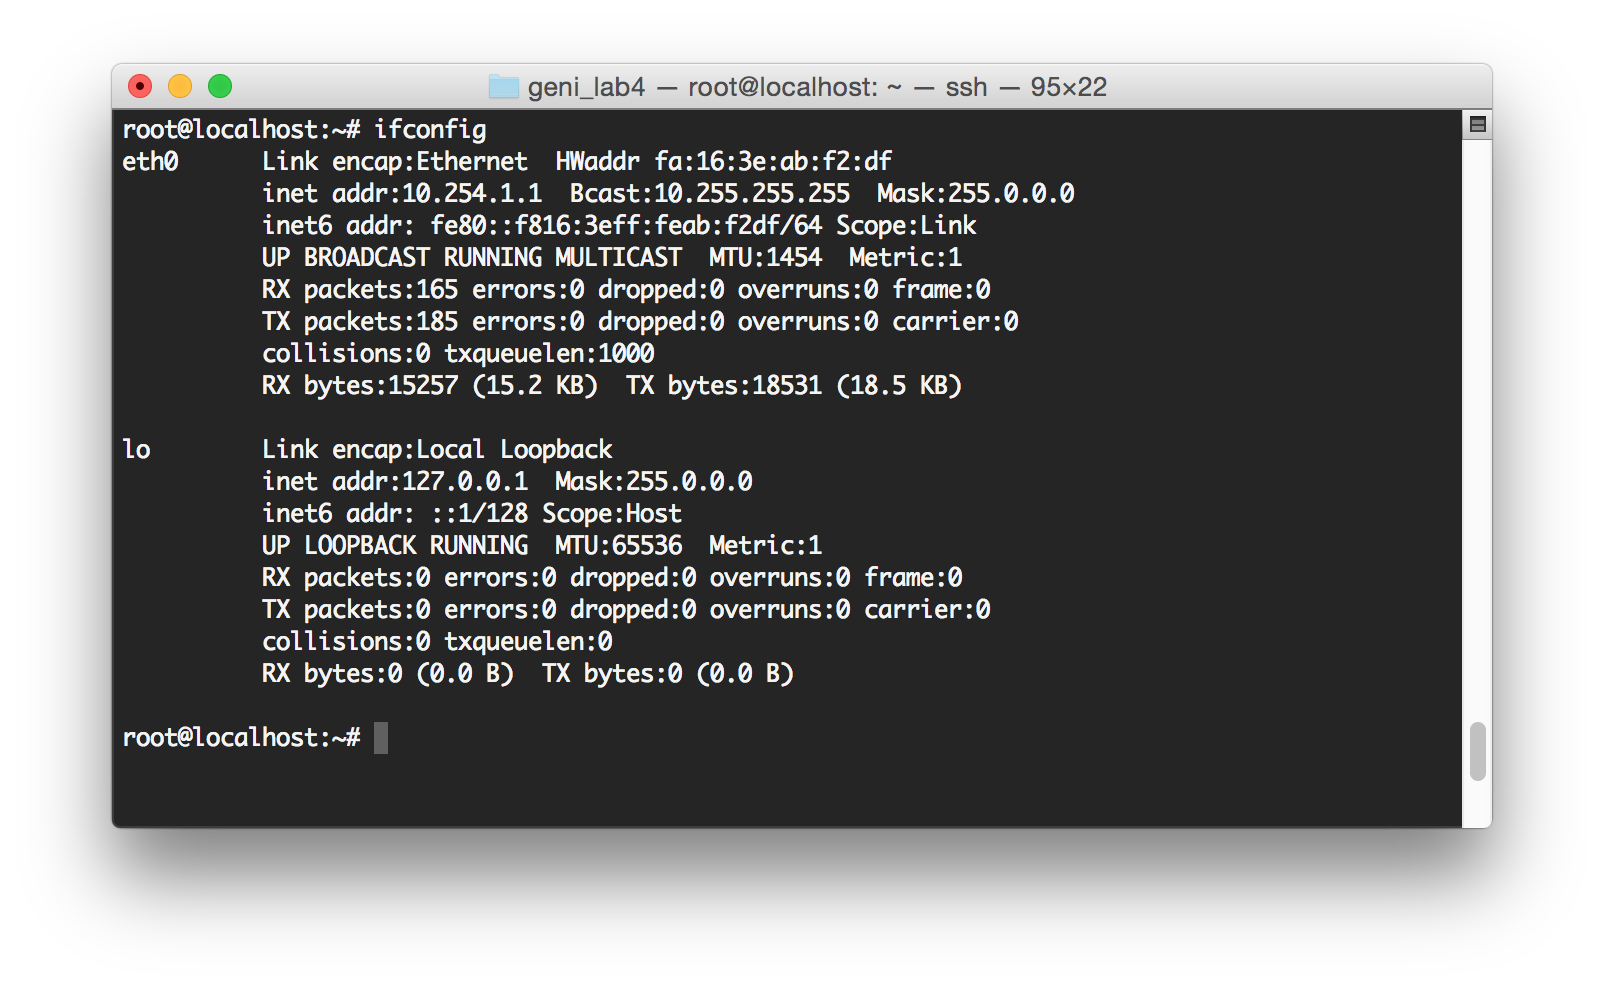
\includegraphics[scale=.54]{mac_address.png}
  \caption{Controller node's MAC address}
\end{figure}

% ---------------------------------------- 3 ----------------------------------------
\paragraph{3. } List in detail the resources available for the deployed cloud infrastructure (vCPUs, RAM, Floating IPs, Security Groups, and Volumes)

% ---------------------------------------- 4 ----------------------------------------
\paragraph{4. } List the necessary changes in the profile file to add an extra compute node, and submit a revised RSpec.

% ---------------------------------------- 5 ----------------------------------------
\paragraph{5. } Extend the Intercloud API to display user list (KEYSTONE) as:
curl -u clouduser:EasyPassword15 \-i http://[IP]:8090/list\_user Provide screenshot of the output.

% ---------------------------------------- 5 ----------------------------------------
\paragraph{6. } By using your AWS instance setup in AWS Lab\-2, you should write a web service client (use any language of your preference) to request and display the cloud information available in the JSON file in a simple web site. Include the Amazon DNS link and the code in your submission report.

\end{document}